% ---------------------------------------------------------------------------- $
\subsection{Versuchsanordnung}
\label{subsec:versuchsanordnung}
% ---------------------------------------------------------------------------- $

%Schema der Versuchsanordnung mit Tabelle der relevanten Daten betreffend Apparatur und
%Umwelt (Geräteliste)

% ---------------------------------------------------------------------------- $
\subsection{Messvorgang/Messmethoden}
\label{subsec:messvorgang}
% ---------------------------------------------------------------------------- $

%mit genauer Bezeichnung der Messgeräte und ihrer Messgenauigkeit, sofern diese nicht
%schon unter 2.1 aufgeführt sind.

% ---------------------------------------------------------------------------- $
\subsection{Proben/Versuchsobjekte}
\label{subsec:proben}
% ---------------------------------------------------------------------------- $

%Beschreibung, sofern nötig, und Tabelle der Daten mit Fehlergrenzen.

% ---------------------------------------------------------------------------- $
\subsection{Messungen}
\label{subsec:messungen}
% ---------------------------------------------------------------------------- $

%Versuchsparameter, allfällige Beobachtungen, Spezialitäten, Finessen.
%In einem "normalen" Laborjournal werden an dieser Stelle die Messergebnisse notiert. Die
%bei uns verwendeten Messprotokollblätter werden zugunsten der Lesbarkeit im Anhang
%abgelegt - umfangreiche Datensätze werden auf CD gebrannt und beigelegt.

% ---------------------------------------------------------------------------- $
\subsubsection{Justierung der Apparatur}
\label{subsubsec:justierung}
% ---------------------------------------------------------------------------- $


% ---------------------------------------------------------------------------- $
\subsubsection{Schnittwinkel der Laserstrahlen}
\label{subsubsec:varphi}
% ---------------------------------------------------------------------------- $

\begin{minipage}[t]{\textwidth}
    \centering
    \resizebox{.75\textwidth}{!}{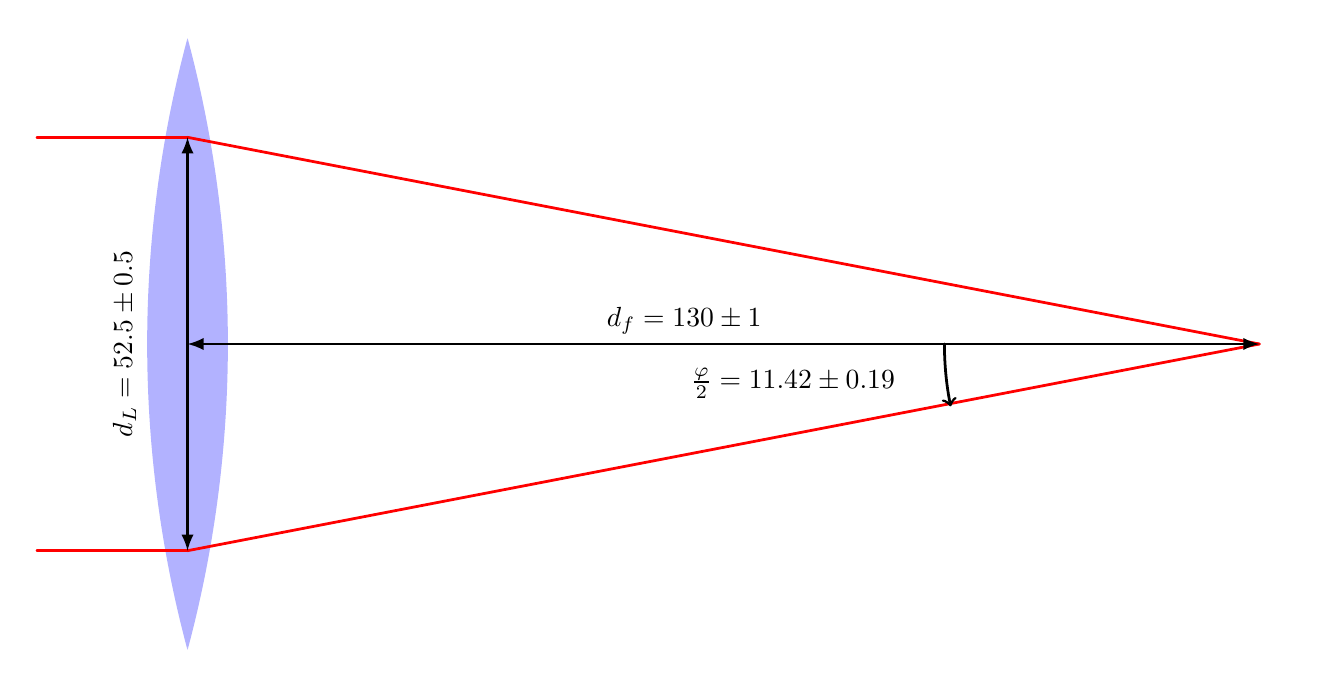
\begin{tikzpicture}
    \begin{scope}[x={(0mm,160mm)},y={(-40mm,40mm)},line width=1pt,cap=round]
        % bounding box
        \draw[white] (0mm,-40mm) rectangle (160mm,40mm);
        %\draw[-] (0mm,-30mm) -- (150mm,30mm);

        % Lens. Center: 20.125mm,0mm
        \fill[-,blue!30] (15mm,   0mm) -- (25.25mm,0mm) arc[start angle=0,  delta angle=15, radius=150mm] -- cycle;
        \fill[-,blue!30] (15mm,   0mm) -- (25.25mm,0mm) arc[start angle=0,  delta angle=-15,radius=150mm] -- cycle;
        \fill[-,blue!30] (25.25mm,0mm) -- (15mm,   0mm) arc[start angle=180,delta angle=15, radius=150mm] -- cycle;
        \fill[-,blue!30] (25.25mm,0mm) -- (15mm,   0mm) arc[start angle=180,delta angle=-15,radius=150mm] -- cycle;

        % incoming laser beams
        \draw[-,red] (1mm, 26.25mm) -- (20.125mm, 26.25mm);
        \draw[-,red] (1mm,-26.25mm) -- (20.125mm,-26.25mm);

        % outgoing laser beams
        \draw[-,red] (20.125mm, 26.25mm) -- (156.25mm,0mm);
        \draw[-,red] (20.125mm,-26.25mm) -- (156.25mm,0mm);

        % measurement arrow
        \draw[latex-latex,black] (20.125mm,0mm) -- (156.25mm,0mm);
        \draw[latex-latex,black] (20.125mm,-26.25mm) -- (20.125mm,26.25mm);
        \node[rotate=90] at (12.125mm,0mm) {$ d_L = \SI{52.5 \pm 0.5}{\milli\meter}$};
        \node at (83.2mm,3mm) {$ d_f = \SI{130 \pm 1}{\milli\meter}$};

        % angle arc
        \draw[->] (116.25mm,0mm) arc[start angle=180, delta angle=11.41, radius=40mm];
        \node at (97mm,-5mm) {$\frac{\varphi}{2} = \SI{11.42 \pm 0.19}{\degree}$};
    \end{scope}
\end{tikzpicture}
}
    \captionof{figure}{%
        Bestimmung des Schnittwinkels der  Laserstrahlen aus der Geometrie der
        Versuchsanordnung.  \emph{Beachte:} Da  diese Abbildung  prim\"ar  der
        Illustration  der Bestimmung  von  $\varphi$ und  nicht der  akkuraten
        Darstellung der Linse  dient, ist hier nicht das  gleiche Symbol f\"ur
        die Linse wie in der Versuchsanleitung benutzt worden.%
    }
    \label{fig:varphi}
\end{minipage}

F\"ur  den Winkel  $\frac{\varphi}{2}$ wurde  die Geometrie  der Laserstrahlen
ausgemessen: Die Distanz $d_L$ zwischen den  beiden Strahlen beim Eintreten in
die Linse und die Distanz $d_f$  zwischen der Linse und dem Kreuzungspunkt der
Laserstrahlen. Die Bestimmung des Schnittwinkels ist  dann nur noch eine Sache
von ein wenig Trigonometrie.

F\"ur   die  Distanzen   ergaben  sich   folgende  Werte,   mit  gesch\"atzten
Unsicherheiten:

\begin{itemize}
    \item
        $ d_L = \SI{52.5 \pm 0.5}{\milli\meter}$
    \item
        $ d_f = \SI{130 \pm 1}{\milli\meter}$
\end{itemize}

Der halbe Schnittwinkel ergibt sich dann zu:

\begin{equation}
    \label{eq:varphi_half}
    \frac{\varphi}{2} = \arctan \frac{\frac{d_L}{2}}{d_f}
\end{equation}

Der kleinstm\"ogliche Winkel ergibt sich aus der Kombination von
$d_L = \SI{52}{\milli\meter}$
und
$d_f = \SI{131}{\milli\meter}$
und
bel\"auft sich auf
$\frac{\varphi}{2} = \SI{11.23}{\degree}$,
der gr\"osstm\"ogliche Winkel korrespondiert mit
$d_L = \SI{53}{\milli\meter}$
und
$d_f = \SI{129}{\milli\meter}$
und ergibt
$\frac{\varphi}{2} = \SI{11.61}{\degree}$,
was sich zusammenf\"uhren l\"asst auf einen Schnittwinkel von:

\begin{equation}
    \label{eq:varphi_result}
    \varphi = \SI{11.42 \pm 0.19}{\degree} \cdot 2 = \SI{22.8 \pm 0.4}{\degree}
\end{equation}

Die   Bestimmung   von   $\varphi$   ist   schematisch   auch   in   Abbildung
\ref{fig:varphi} dargestellt.
